\chapter{機電系統}
\section{Arduino Mega 2560}
\begin{figure}[hbt!]
\begin{center}
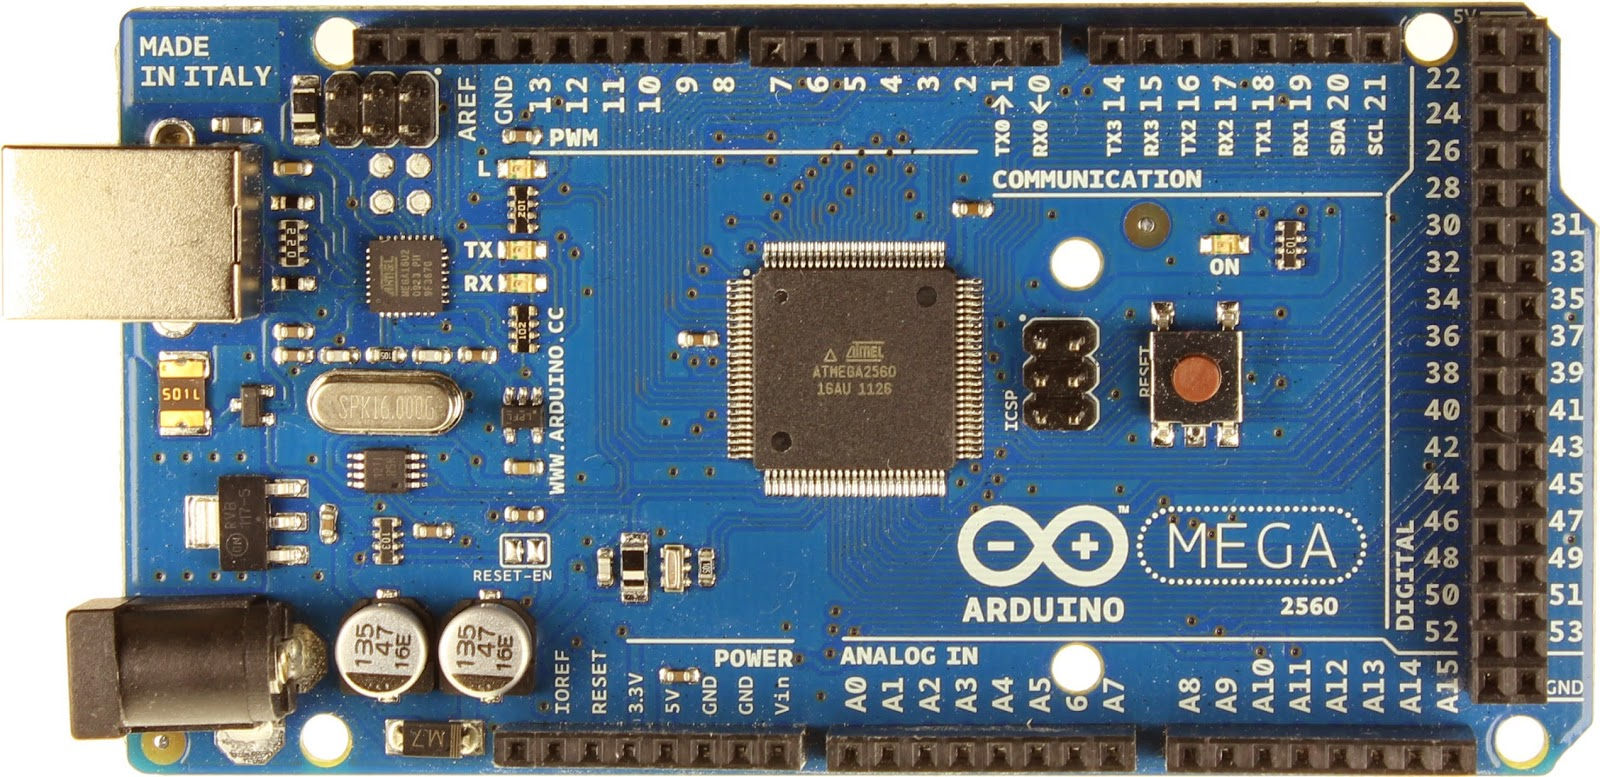
\includegraphics[width=16cm]{ArduinoMega2560}
\caption{\Large Arduino Mega 2560}\label{ArduinoMega2560}
\end{center}
\end{figure}
 Arduino Mega 2560 是基於ATmega2560的主控開發板。Arduino Mega 2560是採用USB接口的核心電路板。它具有54個數位輸入輸出,適合需要大量複雜I/O接口的設計。核心處理器為ATmega2560,它同時具有54路數位輸入/輸出口、16個類比輸入,4個UART接口、1個16MHz晶體振盪器、1個USB連接口、1個電源插孔、1個ICSP接頭以及1個復位按鈕。Arduino Mega 2560也能兼容爲Arduino NUO設計的擴展板。可以自動選擇3中供電方式:外部直流電源通過電源插座供電;電池連接電源連接器的GND和VIN引腳;USB接口直流供電,整合了微控制器以及燒錄功能於一身。\\[6pt]

\section{RAMPS 1.4}
 RAMPS 1.4 為RepRep Arduino Mega Pololu Shield的縮寫,主要為設計給步進馬達驅動器的介面電路,1.4為電路版本號碼,目前最新版本為1.7,Arduino Mega 2560可透過RAMPS 1.4介面與控制電路溝通進而達成控制步進馬達以及其他硬體的功能,目前可控制X、Y、Z三軸與最多兩個擠出頭以及兩個散熱風扇。\\


\newpage 